%# -*- coding: utf-8-unix -*-
% !TEX program = xelatex
% !TEX root = ../thesis.tex
% !TEX encoding = UTF-8 Unicode
%%==================================================
%% chapter02.tex for SJTU Master Thesis
%% based on CASthesis
%% modified by wei.jianwen@gmail.com
%% Encoding: UTF-8
%%==================================================

\chapter{Modeling and Analysis}
\label{chap:modeling and analysis methods}

\section{Modeling of two layer network}
\label{sec:modeling of two layer network}

The model consists of two layers, and each layer has different dynamics. For layer A, the node change its states according to $M$ model as introduced in \cite{rocca2014}. Here, we choose $M=2$, that each node has four states $(-2, -1, +1, +2)$. For each link $(k, j)$ belong to layer A,  the dynamics are designed as follows:
\begin{itemize}
	\item Compromise : if two nodes connected with link$(k, j)$ have opposite orientations, their states become more moderate with probability $q$ :
	\begin{align}
	\mbox{if } S_k<0 \mbox{ and } S_j>0  \Rightarrow (S_k, S_j) \rightarrow (S_k^r, S_j^l) \mbox{ with } prob.q,\\
	\mbox{if } S_k>0 \mbox{ and } S_j<0  \Rightarrow (S_k, S_j) \rightarrow (S_k^l, S_j^r) \mbox{ with } prob.q.
	\end{align}
	If $S_k = \pm1$ and $S_j = \mp1$, one switches orientation at random:
	\begin{align}
	(\pm 1, \mp 1)\rightarrow \left\{\begin{matrix}
	(+1, +1) \mbox{ with } prob.q/2,
	\\(-1, -1)\mbox{ with } prob.q/2.
	\end{matrix}\right.
	\end{align}
	\item Persuasion : if two nodes connected with link$(k, j)$ have the same orientation, their states become more extreme with probability $p$ :
	\begin{align}
	\mbox{if } S_k<0 \mbox{ and } S_j<0  \Rightarrow (S_k, S_j) \rightarrow (S_k^l, S_j^l) \mbox{ with } prob.p,\\
	\mbox{if } S_k>0 \mbox{ and } S_j>0  \Rightarrow (S_k, S_j) \rightarrow (S_k^r, S_j^r) \mbox{ with } prob.p.
	\end{align}
\end{itemize}
For each external link $(k,j)$ with $k$ belong to layer A, the state of node $k$ is updated according to :
\begin{itemize}
	\item $S_k \cdot S_j < 0$ :
	\begin{align}
	\mbox{if } S_k<0 \mbox{ and } S_j>0  \Rightarrow (S_k, S_j) \rightarrow (S_k^r, S_j) \mbox{ with } prob.q,\\
	\mbox{if } S_k>0 \mbox{ and } S_j<0  \Rightarrow (S_k, S_j) \rightarrow (S_k^l, S_j) \mbox{ with } prob.q.
	\end{align}
	\item $S_k \cdot S_j > 0$ :
	\begin{align}
	\mbox{if } S_k<0 \mbox{ and } S_j<0  \Rightarrow (S_k, S_j) \rightarrow (S_k^l, S_j) \mbox{ with } prob.p,\\
	\mbox{if } S_k>0 \mbox{ and } S_j>0  \Rightarrow (S_k, S_j) \rightarrow (S_k^r, S_j) \mbox{ with } prob.p.
	\end{align}
\end{itemize}
Here, $S_k^r$ and $S_k^l$ denote the right and left neighboring states of $k$, defined as
\begin{align}
S_k^r &= \left\{\begin{matrix}
+1,\mbox{ for } S_k = -1\\
+2,\mbox{ for } S_k = +2\\ 
S_k + 1,\mbox{ otherwise }, 
\end{matrix}\right. &
S_k^l &= \left\{\begin{matrix}
-1,\mbox{ for } S_k= +1
\\ -2,\mbox{ for } S_k=-2
\\ S_k - 1,\mbox{ otherwise }.
\end{matrix}\right.
\end{align}

The sign of $S^A$ represents its opinion orientation and its absolute value $|S^A|$ measures the intensity of its opinion. So, $|S^A|=2$ represents to a positive or a negative extremist, while  $|S^A|=1$ correspond to a moderate opinion of each side. In case of internal link $(k, j)$ belong to layer A, when the nodes have the same orientation$(S_kS_j>0)$, if the states of nodes are moderate, then they become extreme$(S_k=\pm1 \rightarrow \pm2, S_j= \pm1 \rightarrow \pm2)$ with probability $p$. If they are already extreme, they remain extreme$(S_k=\pm2 \rightarrow \pm2, S_j= \pm2 \rightarrow \pm2)$. On the other hand, when the nodes have opposite orientations$(S_kS_j<0)$, if they are extreme, the states of nodes become moderate$(S_k=\pm2 \rightarrow \pm1, S_j= \pm2 \rightarrow \pm1)$ with probability $q$. If they are already moderate, they switch orientations individually$(S_k=\pm1 \rightarrow \mp1, S_j= \pm1 \rightarrow \mp1)$.  In case of interaction between node in layer A and node in layer B, node in layer A follows opinion dynamics formula, but the state of node in layer B does not change. In other words, the state of layer B affects layer A, but layer A dynamics does not affect the state of node in layer B. For example, one of the layer A node, $S_k = +2$ is connected with  $S_j = -1$ node of layer B. Here, $S_k$ will change into $S_k = +1$ with $prob.q$. But $S_j$ will not change, which indicates that the states of layer B will influence the states of layer A.

The dynamics of layer B follows the decision-making dynamics as introduced in \cite{abrams2003, vazquez2010}. The state of node i in layer B can be $+1$ and $-1$, and it updates according to

\begin{equation}
{P_B}({S_i} \to  - {S_i}) = \begin{cases}
{\left({\displaystyle\frac{{{i_i} + {e_i}}}{{{n^{ - {S_i}}}}}}\right)}{\cdot}{\left({\displaystyle\frac{{n^{-{S_i}}}}{{{i_i} + {e_i}}}} \right)^{1/v}}  ,\mbox{ if } v \ne 0\\
0,\mbox{ if } v = 0\\
0,\mbox{ if } {n^{ - {S_i}}} = 0
\end{cases},
\end{equation}

where $i_i$ is the number of internal edges and $e_i$ is the number of external edges. $n^{-S_i}$ is the number of neighbors of i with opposite state $-S_i$. $v$ represents the volatility that measures how prone a node change its state. The scale of $v$ is from $0$ to $1$. If $v \simeq 0$,  a node is unlikely to change its state. On the other hand, if $v \simeq 1$, a node is very likely to change its state. Also, this formula shows that the more the number of nodes connected with the opposite state is, the easier the nodes are to change into the opposite state.\\
\begin{figure}[!htb]
	\centering
	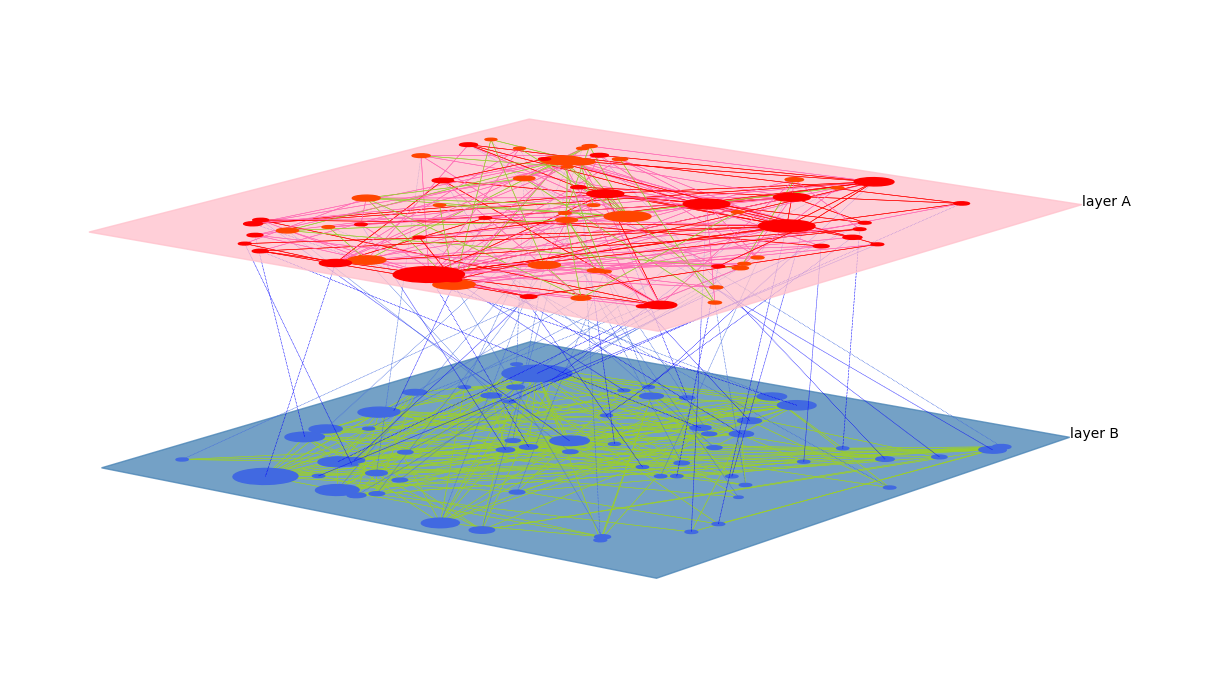
\includegraphics[width=\hsize]{FIG1.png}
	\caption{Competition of Interconnected Network}
	\label{Fig1}
\end{figure}

\section{Simulations and Analysis}
To start with a polarized competition, as the initial conditions,  nodes in layer A are all positive, and nodes in layer B are all negative as shown in Fig.~\ref{Fig1}. For nodes in layer A, it begins with the status where half of nodes are $+1$ and the others are $+2$. The initial state of nodes in layer B have only $-1$. 

There are two parameters in the dynamics of layer A. To simply represent the probability $p$ and probability $q$ together, we set $p+q=1$. So, $p$ represents the tendency of opinion such as extreme or moderate, which is scaled to be $0$ to $1$. And, the scale of $v$, in the dynamics of layer B, is also $0$ to $1$. 

To implement the interconnected dynamics, one step consists of two layers dynamics, where every node in layer A will be checked with opinion dynamics, and every node in layer B will updates its state according to the decision-making dynamics. Here, we would control dynamics orders between layers and updating rules of nodes states. With changing dynamics orders and updating rules, it would be investigated how state of network change.      

Each simulation takes $100$ steps, and $100$ simulations are considered for average results. In the following simulations, we use \textit{`Average State'(AS)} and \textit{`Consensus Index'(CI)} to measure the competition result.

\begin{equation}
AS = avg\left( {\sum\limits_i^{{K^A}} {S_i^A/4} } \right) + avg\left( {\sum\limits_i^{{K^B}} {S_i^B/2} } \right).
\end{equation}

\begin{equation}
CI = \frac{{({K_ + }^A \cdot {K_ - }^B) + ({K_ - }^A \cdot {K_ + }^B)}}{{{K^A} \cdot {K^B}}}
\end{equation}

In these formula, $S_i^A$ means the state of node \textit{i} in layer A, and $K^A$ is the number of nodes in layer A. ${K_ + }^A$ represents the number of nodes with positive state in layer A.   

With \textit{AS}, it could be verified whether the consensus happens in accordance with the change of $p$ and $v$.  If the positive consensus happens, it would be close to the value of $+1$ and if the negative consensus happens, it would be close to the value of $-1$. The values between $+1$ and $-1$ mean the states are belonging to the coexistence part.

With \textit{CI}, it could be measured how close the network state is to consensus. If the CI is close to $0$, the state is close to positive or negative consensus. If the CI is close to $1$, the state is separated coexistence where states of all nodes in layer A is opposed to states of all nodes in layer B. If the CI is close to $0.5$, the state is mixed coexistence where each layer has both positive and negative states of nodes.    

\begin{figure*}[!htb]
	\centering
	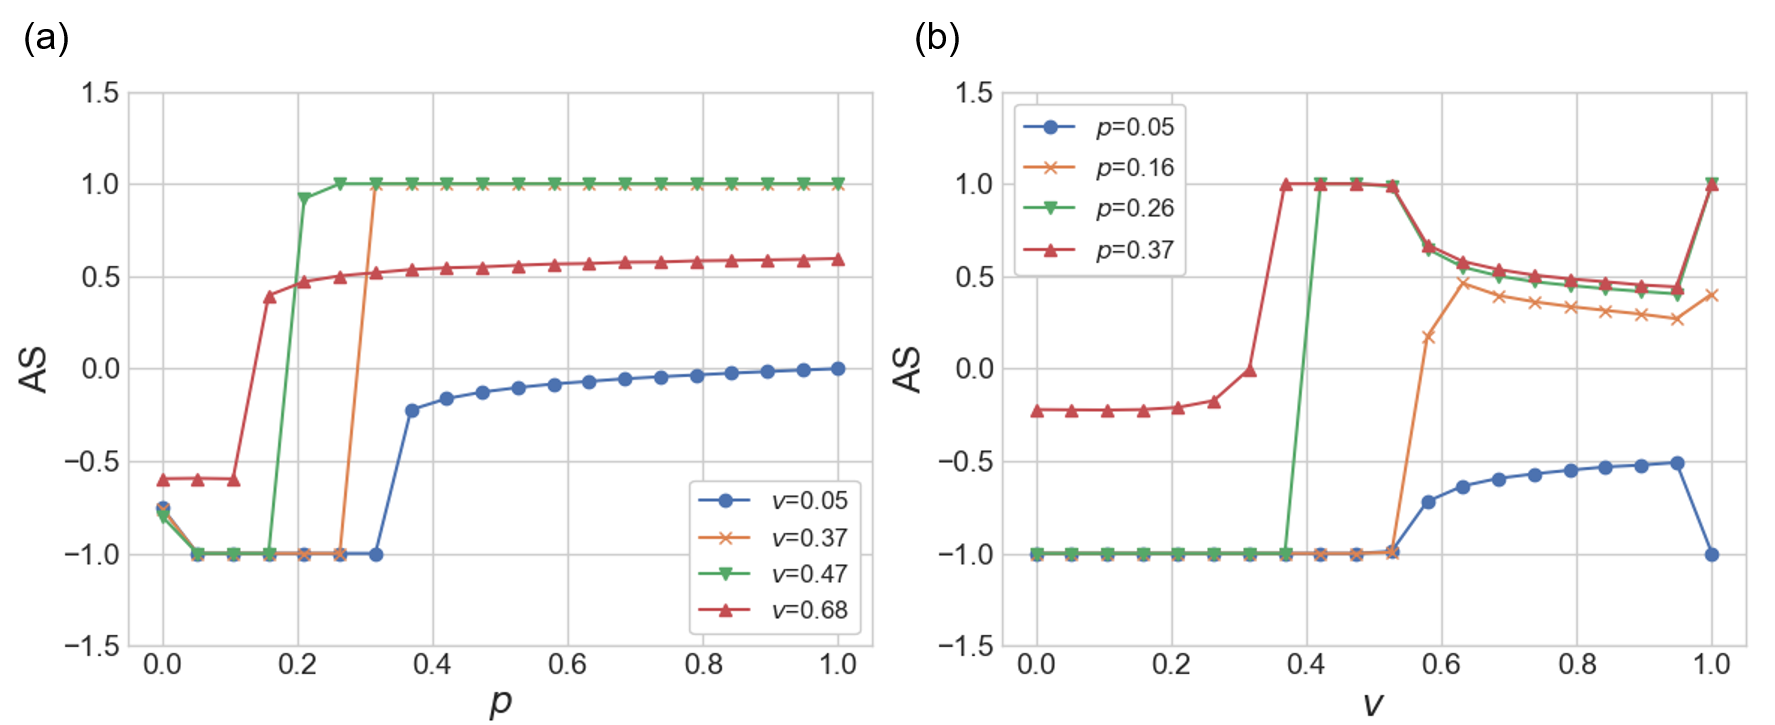
\includegraphics[width=\hsize]{AS_2d.png}
	\caption{(a) $p$-\textit{AS} chart according to certain $v$ values. (b) $v$-\textit{AS} chart according to certain $p$ values.}
	\label{AS_2d}
\end{figure*}

\begin{figure}[!htb]
	\centering
	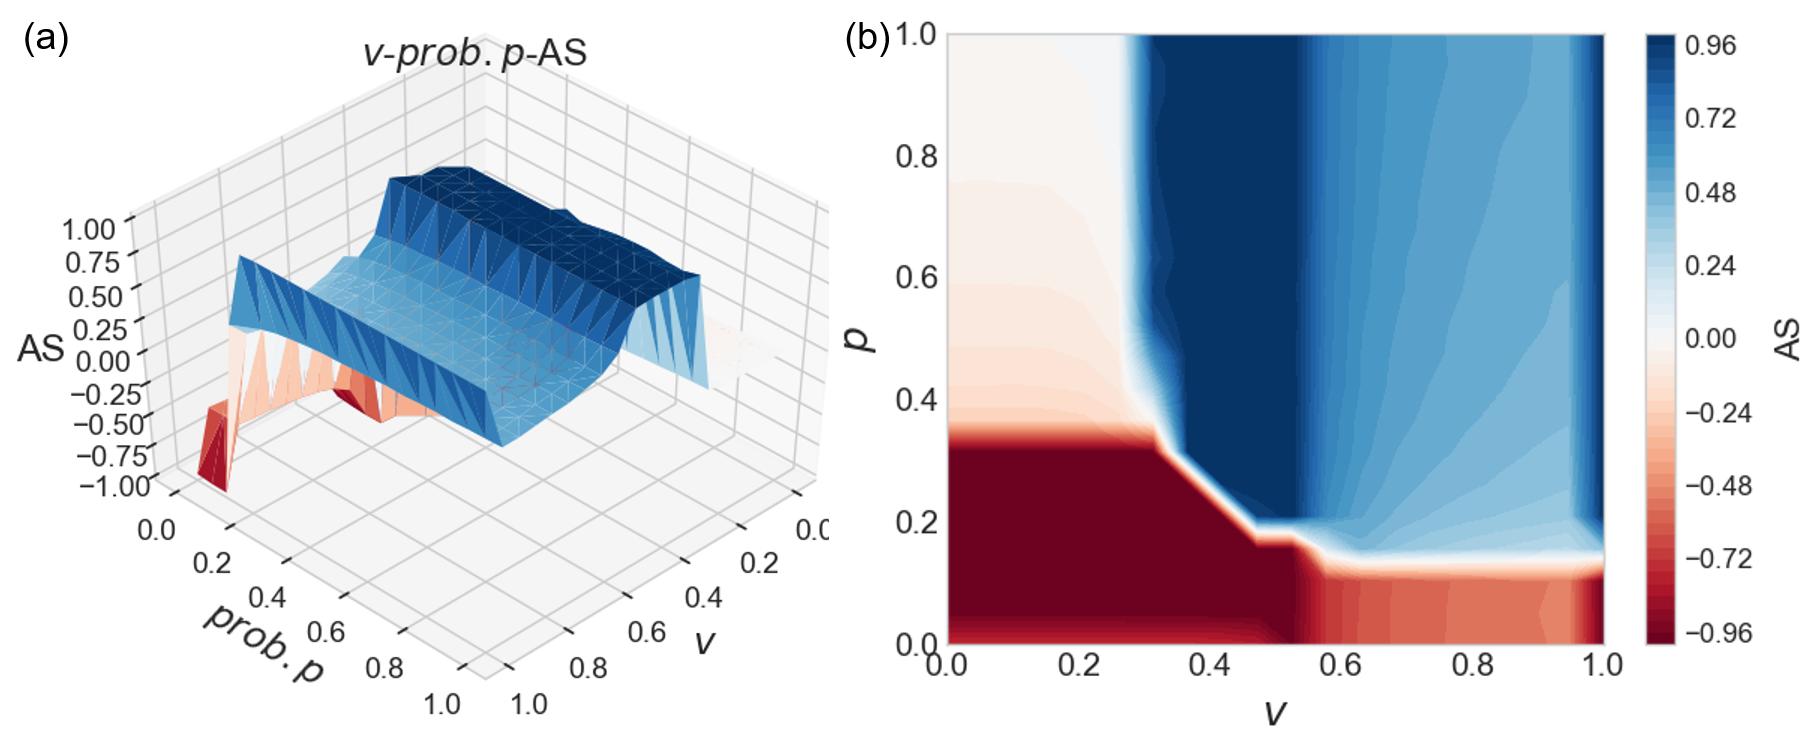
\includegraphics[width=\hsize]{p_v_AS_3d.png}
	\caption{Two layer networks with sequential updating rule : \textit{AS} changing with all $p$ and $v$}
	\label{p_v_AS_3d}
\end{figure}



\chapter{Competition on two layer with different structural network}
\label{chap:competition on two layer with different structural network}


\section{Competition on Networks with different number of external links}

In this subsection, we consider the influence of external links. Based on the basic model in Subsection 3.1, we reduce the number of nodes in layer B at a certain rate and increase the external links from nodes in layer B accordingly.  We denote \textit{HM(n)} as a hierarchical model with a level $n$, which means that the number of nodes in layer B is $1/n$ of the number of nodes in layer A, and the number of external links from node in layer B is $n$ in view that the number of external links from node in layer A is $1$. In other words, each node in layer A has one external edge, but each node in layer B has $n$ external edges for \textit{HM(n)}, which means one node in layer B can be influenced by $n$ nodes in layer A. $\gamma$ scale is same as the Random Regular Networks Model. But, $\beta$ scale depends on the number of degrees. So the $\beta$ scale is adjusted to have the same probability of volatility with Random Regular Networks Model(\textit{RRM}) as following Equation.
\begin{equation}
{\beta _{h,\max}} = {\beta _{rr,\max}} \cdot \log \left( {\frac{{{n_{rr}}^{ - {S_i}}}}{{{i_{rr,i}} + {e_{rr,i}}}} \cdot \frac{{{i_{h,i}} + {e_{h,i}}}}{{{n_{h}}^{ - {S_i}}}}} \right). 
\end{equation}

Eq(6) is derived from Eq(1) at the initial states. $\beta _{h,\max}$ is the maximum value of $\beta$ scale in \textit{HM}, and $\beta _{rr,\max}$ is the maximum value of $\beta$ scale in \textit{RRM}. When \textit{RRM} begins with initial state and the maximum of $\beta$ scale, it has the lowest volatility except $0$. In order to have the same probability in layer B dynamics for different network structures at the initial time, maximum value of $\beta$ in \textit{HM} is calculated based on Eq(6). 

Fig.~\ref{Fig4} shows the Hierarchical Model simulation results. Comparing \textit{HMs} with \textit{RRM}, \textit{CR} and \textit{PCR} are all increased remarkably. \textit{HMs} have more positive consensus part than \textit{RRM}. It shows that as the number of B nodes are decreased, it is easy to make positive consensus. Comparing \textit{HM(16)} with other \textit{HMs}, \textit{HM(16)} has the most positive consensus part. In case of models where the number of nodes in layer B is less than \textit{HM(16)},  \textit{CR} and \textit{PCR} of the models are decreased and \textit{NCR} is increased slightly. Also, for models where the number of nodes in layer B is more than \textit{HM(16)}, \textit{CR} and \textit{PCR} are also decreased. However, \textit{HM(4)} has the most \textit{AS total}. Although \textit{HM(4)} doesn't have the most consensus part, it has more intensity for positive social opinion. It can be analyzed that strong social intensity usually can not make more consensus. These results indicate that network structure can contribute more for consensus. 

\begin{figure}[!htb]
	\centering
	\includegraphics[width=\hsize]{FIG4.png}
	\caption{Hierarchical Model(\textit{HM(n)})}
	\label{Fig4}
\end{figure}

In summary, all the Hierarchical Models have more consensus ratio than Random Regular Networks Model. Among \textit{HMs}, \textit{HM(16)} has the most positive consensus part. When the number of nodes in layer B is more or less than \textit{HM(16)}, \textit{CR} and \textit{PCR} are decreased. This shows that there exists an efficient number for the decision making layer to perform positive consensus.  

\section{Competition on Networks with different number of internal links}
\begin{figure}[!htb]
	\centering
	\includegraphics[width=\hsize]{FIG5.png}
	\caption{Comparison of Networks with different internal degrees(\textit{RR(n)-RR(m)}: layer A has random regular network with $n$ internal edges, layer B has random regular network with $m$ internal edges)}
	\label{Fig5}
\end{figure}
Next, the interconnected networks are simulated with different internal degrees in order to define and evaluate the influence of internal degrees. The number of internal degrees on each node is switched to $2$ or $5$.

Fig.~\ref{Fig5} shows the simulation results with changing the number of internal edges. \textit{RR(5)-RR(2)} has the most \textit{PCR}. \textit{RR(2)-RR(5)} has the most \textit{NCR}. When the number of internal edges in layer A are more than layer B, it has more positive consensus. On the other hand, when the number of internal edges in layer B are more than layer A, it has relatively more negative consensus. These results provide that the number of edges on layer A has the tendency to keep positive state, and the number of edges on layer B has the tendency to keep negative state. The number of internal edges have the influence on consensus result and a layer with more internal edges has the tendency to maintain its own state. In case of networks with same internal edges, \textit{RR(2)-RR(2)} has more \textit{PCR} and \textit{AS total} than \textit{RR(5)-RR(5)}. It can be analyzed that \textit{RR(5)-RR(5)} is hard to make consensus, because it has more internal edges to cause inner conflict. Also, \textit{RR(2)-RR(2)} has less \textit{NCR} than \textit{RR(5)-RR(5)}. It shows that the number of internal edges in layer B is more sensitive than layer A. As Eq(1) shows, layer B dynamics can have more various and extreme probabilities when it has more degrees. For example, in case of \textit{RR(2)-RR(2)} with $\beta = 1$, the dynamics starts with $P_B=1/3$ and in case of \textit{RR(5)-RR(5)} with $\beta = 1$, the dynamics starts with $P_B=1/6$.    

\section{Competition on Networks with different structures}
So far, each layer of the interconnected network consisted of random regular networks that has the same number of edges for each node. Now, the simulation would be implemented on different network structures. 

\begin{figure}[!htb]
	\centering
	\includegraphics[width=\hsize]{FIG6.png}
	\caption{Comparison of Networks with different structures}
	\label{Fig6}
\end{figure}

Here, we use \textit{Barabasi-Albert network(BA)} structure as introduced in \cite{barabasi1999}. To evaluate the influence of network structure, 5 simulations are implemented with changing network structures. The \textit{BA} network is applied for both layers or switched on each layer. And, because layer A with \textit{BA} network structure has total $10,215$ internal edges, \textit{RR(10)-RR(5)}, under the similar conditions such as the number of nodes and edges, is also simulated. The simulation results are shown in Fig.~\ref{Fig6}. The result of \textit{BA-RR} and \textit{RR(10)-RR(5)} have almost the same features. The gap of \textit{CR} is almost same(less than 0.01). The structure of network make no obvious difference of consensus results. In case of \textit{BA-BA}, the \textit{CR} has the least ratio for consensus. \textit{BA-BA} structure has lots of internal edges on each layer. Therefore, it is hard to make consensus due to inner conflict on each layer. 
